\begin{singlespace}
\chapter{\textbf{Root mass carbon costs to acquire nitrogen are determined by nitrogen and light availability in two species with different nitrogen acquisition strategies}}
\end{singlespace}

\begin{singlespace}
    \noindent Perkowski EA, EF Waring, NG Smith, ``Root mass carbon costs to acquire nitrogen are determined by nitrogen and light availability in two species with different nitrogen acquisition strategies'', \textit{Journal of Experimental Botany}, 2021, Volume 72, Issue 15, Pages 5766-5776, by permission of Oxford University Press
\end{singlespace}

\bigskip
\section{Introduction}
\noindent Carbon and nitrogen cycles are tightly coupled in terrestrial ecosystems. This tight coupling influences photosynthesis \shortcite{Walker2014,Rogers2017a}, net primary productivity \shortcite{LeBauer2008,Thomas2013}, decomposition \shortcite{Cornwell2008,Bonan2013,Sulman2019}, and plant resource competition \shortcite{Gill2016,Xu-Ri2017}. Terrestrial biosphere models are beginning to include connected carbon and nitrogen cycles to improve the realism of their simulations \shortcite{Fisher2010,Brzostek2014FUN2,Wieder2015_NPP,Shi2016,Zhu2019}. Simulations from these models indicate that coupling carbon and nitrogen cycles can influence future biosphere-atmosphere feedbacks under global change, such as elevated carbon dioxide or nitrogen deposition \shortcite{Thornton2007,Goll2012,Wieder2015_NPP,Wieder2019}. Nonetheless, there are still limitations in our quantitative understanding of connected carbon and nitrogen dynamics \shortcite{Thomas2015,Meyerholt2016,Rogers2017a,Exbrayat2018,Shi2019}, forcing models to make potentially unreliable assumptions.

Plant nitrogen acquisition is a process in terrestrial ecosystems by which carbon and nitrogen are tightly coupled \shortcite{Vitousek1991,Delaire2005,Brzostek2014FUN2}. Plants must allocate carbon belowground to produce and maintain root systems or exchange with symbiotic soil microbes in order to acquire nitrogen \shortcite{Hogberg2007,Hogberg2010}. Thus, plants have an inherent carbon cost associated with acquiring nitrogen, which can include both direct energetic costs associated with nitrogen acquisition and indirect structural costs associated with allocation \shortcite{Gutschick1981,Rastetter2001,Vitousek2002,Menge2008}. Model simulations \shortcite{Fisher2010,Brzostek2014FUN2,Shi2016,Allen2020} and meta-analyses \shortcite{Terrer2018} suggest that these carbon costs vary between species, particularly those with different nitrogen acquisition strategies. For example, simulations using iterations of the Fixation and Uptake of Nitrogen (FUN) model indicate that species that acquire nitrogen from non-symbiotic active uptake pathways (e.g., mass flow) generally have larger carbon costs to acquire nitrogen than species that acquire nitrogen through symbiotic associations with nitrogen-fixing bacteria \shortcite{Brzostek2014FUN2,Allen2020}.

Carbon costs to acquire nitrogen likely vary in response to changes in soil nitrogen availability. For example, if the primary mode of nitrogen acquisition is through non-symbiotic active uptake, then nitrogen availability could decrease carbon costs to acquire nitrogen as a result of increased per-root nitrogen uptake \shortcite{Franklin2009,Wang2018}. However, if the primary mode of nitrogen acquisition is through symbiotic active uptake, then nitrogen availability may incur additional carbon costs to acquire nitrogen if it causes microbial symbionts to shift toward parasitism along the parasitism–mutualism continuum \shortcite{Johnson1997,Hoek2016,Friel2019} or if it reduces the nitrogen acquisition capacity of a microbial symbiont \shortcite{VanDiepen2007,Soudzilovskaia2015,Munoz2016}. Species may respond to shifts in soil nitrogen availability by switching their primary mode of nitrogen acquisition to a strategy with lower carbon costs to acquire nitrogen in order to maximize the magnitude of nitrogen acquired from a belowground carbon investment and outcompete other individuals for soil resources \shortcite{Rastetter2001,Menge2008}.

Environmental conditions that affect plant nitrogen demand (e.g., CO$_2$, light availability) could also affect plant carbon costs to acquire nitrogen.  For example, an increase in plant nitrogen demand could increase carbon costs to acquire nitrogen if this increases the carbon that must be allocated belowground to acquire a proportional amount of nitrogen \shortcite{Kulmatiski2017,Noyce2019}. This could be driven by a temporary state of diminishing return associated with investing carbon toward building and maintaining structures that are necessary to support enhanced nitrogen uptake, such as fine roots \shortcite{Matamala2000,Norby2004,Arndal2018}, mycorrhizal hyphae \shortcite{Saleh2020}, or root nodules \shortcite{Parvin2020}. Alternatively, if the environmental factor that increases plant nitrogen demand causes nitrogen to become more limiting in the system (e.g. atmospheric CO$_2$) \shortcite{Luo2004,LeBauer2008,Vitousek2010,Liang2016}, species might switch their primary mode of nitrogen acquisition to a strategy with lower relative carbon costs to acquire nitrogen in order to gain a competitive advantage over species with either different or more limited modes of nitrogen acquisition \shortcite{Ainsworth2005,Taylor2018}.

Using a plant economics approach, I examined the influence of plant nitrogen demand and soil nitrogen availability on plant carbon costs to acquire nitrogen. This was done by growing a species capable of forming associations with nitrogen-fixing bacteria (\textit{Glycine max} L. (Merr)) and a species not capable of forming these associations (\textit{Gossypium hirsutum} L.) under four levels of light availability (plant nitrogen demand proxy) and four levels of soil nitrogen fertilization (soil nitrogen availability proxy) in a full-factorial, controlled greenhouse experiment. These species are commonly used in regional west Texan cropping systems and have fast growth rates, but differ in growth form (\textit{G. hirsutum} is a perennial woody species, \textit{G. max} is an annual herbaceous species). Species were selected as a hypothesis generation exercise to determine whether effects of fertilization and light availability on carbon costs to acquire nitrogen were directionally similar between species, though this selection does limit my ability to deduce mechanisms that drive species differences across treatment combinations. I used this experimental design to test the following hypotheses:
\begin{enumerate}
\item An increase in plant nitrogen demand due to increasing light availability will increase carbon costs to acquire nitrogen through a proportionally larger increase in belowground carbon than whole-plant nitrogen acquisition. This will be the result of an increased investment of carbon toward belowground structures that support enhanced nitrogen uptake, but at a lower nitrogen return. 

\item An increase in soil nitrogen availability will decrease carbon costs to acquire nitrogen as a result of increased per root nitrogen uptake in \textit{G. hirsutum}. However, soil nitrogen availability will not affect carbon costs to acquire nitrogen in \textit{G. max} because of the already high return of nitrogen supplied through nitrogen fixation.
\end{enumerate}

\section{Methods}
\subsection{\textit{Experiment setup}}
\noindent \textit{Gossypium hirsutum} and \textit{G. max}. were planted in individual 3 liter pots (NS-300; Nursery Supplies, Orange, CA, USA) containing a 3:1 mix of unfertilized potting mix (Sungro Sunshine Mix \#2, Agawam, MA, USA) to native soil extracted from an agricultural field most recently planted with \textit{G. max} at the USDA-ARS Laboratory in Lubbock, TX, USA (33.59\textdegree{}N, –101.90\textdegree{}W). The field soil was classified as Amarillo fine sandy loam (75\% sand, 10\% silt, 15\% clay). Upon planting, all \textit{G. max} pots were inoculated with \textit{Bradyrhizobium japonicum} (Verdesian N-Dure\texttrademark\ Soybean, Cary, NC, USA) to stimulate root nodulation. Individuals of both species were grown under similar, unshaded, ambient greenhouse conditions for 2 weeks to germinate and begin vegetative growth. 

Three blocks were set up in the greenhouse, each containing four light treatments created using shade cloth that reduced incoming radiation by either 0 (full sun), 30, 50, or 80\%. Two weeks post-germination, individuals were randomly placed in the four light treatments in each block. Individuals received one of four nitrogen fertilization doses as 100mL of a modified Hoagland solution \shortcite{Hoagland1950} equivalent to either 0, 70, 210, or 630 ppm N twice per week within each light treatment. Nitrogen fertilization doses were received as topical agents to the soil surface. Each Hoagland solution was modified to keep concentrations of other macro- and micronutrients equivalent (Table \ref{table:tab.a1}). Plants were routinely well watered to eliminate water stress.

\subsection{\textit{Plant measurements and calculations}}
\noindent Each individual was harvested after 5 weeks of treatment, and biomass was separated by organ type (leaves, stems, and roots). Nodules on \textit{G. max} roots were also harvested. Except for the 0\% shade cover and 630 ppm N treatment combination, all treatment combinations in both species had lower average dry biomass:pot volume ratios than the 1:1 ratio recommended by \shortciteN{Poorter2012} to minimize the likelihood of pot volume-induced growth limitation (Table \ref{table:tab.a2}, \ref{table:tab.a3}; Fig. \ref{fig:figure.a1}). 

All harvested material was dried, weighed, and ground by organ type. Carbon and nitrogen content (g g$^{-1}$) was determined by subsampling from ground and homogenized biomass of each organ type using an elemental analyzer (Costech 4010; Costech, Inc., Valencia, CA, USA). I scaled these values to total leaf, stem, and root carbon and nitrogen biomass (g) by multiplying dry biomass of each organ type by carbon or nitrogen content of each corresponding organ type. Whole plant nitrogen biomass (g) was calculated as the sum of total leaf (g), stem (g), and root (g) nitrogen biomass. Root nodule carbon biomass was not included in the calculation of root carbon biomass; however, relative plant investment toward root or root nodule standing stock was estimated as the ratio of root biomass to root nodule biomass (g g$^{-1}$), following similar metrics to those adopted by \shortciteN{Dovrat2018} and \shortciteN{Dovrat2020}.

Carbon costs to acquire nitrogen ($N_\mathrm{cost}$; gC gN$^{-1}$) were estimated as the ratio of total root carbon biomass ($C_\mathrm{bg}$; gC) to whole-plant nitrogen biomass ($N_\mathrm{wp}$; gN). This calculation quantifies the relationship between carbon spent on nitrogen acquisition and whole plant nitrogen acquisition by using root carbon biomass as a proxy for estimating the magnitude of carbon allocated toward nitrogen acquisition. This calculation therefore assumes that the magnitude of root carbon standing stock is proportional to carbon transferred to root nodules or mycorrhizae, or lost through root exudation or turnover. The assumption has been supported in species that associate with ectomycorrhizal fungi \shortcite{Hobbie2006,Hobbie2008}, but is less clear in species that acquire nitrogen through non-symbiotic active uptake or symbiotic nitrogen fixation. It is also unclear whether relationships between root carbon standing stock and carbon transfer to root nodules are similar in magnitude to carbon lost through exudation or when allocated toward other active uptake pathways. Thus, because of the way measurements were calculated, proximal values of carbon costs to acquire nitrogen are underestimates.

\subsection{\textit{Statistical analyses}}
\noindent I explored the effects of light and nitrogen availability on carbon costs to acquire nitrogen using separate linear mixed-effects models for each species. Models included shade cover, nitrogen fertilization, and interactions between shade cover and nitrogen fertilization as continuous fixed effects, and also included block as a random intercept term. Three separate models for each species were built with this independent variable structure for three different dependent variables: (i) carbon costs to acquire nitrogen (gC gN$^{-1}$); (ii) whole plant nitrogen biomass (denominator of carbon cost to acquire nitrogen; gN); and (iii) belowground carbon biomass (numerator of carbon cost to acquire nitrogen; gC). I constructed two additional models for \textit{G. max} with the same model structure described above to investigate the effects of light availability and nitrogen fertilization on root nodule biomass (g) and the ratio of root nodule biomass to root biomass (unitless).

I used Shapiro–Wilk tests of normality to determine whether species specific linear mixed-effects model residuals followed a normal distribution. Zero models satisfied residual normality assumptions when models were fit using untransformed data (Shapiro–Wilk: \textit{p}<0.05 in all cases). I attempted to satisfy residual normality assumptions by first fitting models using dependent variables that were natural-log transformed. If residual normality assumptions were still not met (Shapiro–Wilk: \textit{p}<0.05), then models were fit using dependent variables that were square root transformed. All residual normality assumptions were satisfied when models were fit with either a natural-log or square root transformation (Shapiro–Wilk: \textit{p}>0.05 in all cases). Specifically, I natural-log transformed \textit{G. hirsutum} carbon costs to acquire nitrogen and \textit{G. hirsutum} whole-plant nitrogen biomass. I also square root transformed \textit{G. max} carbon costs to acquire nitrogen, \textit{G. max} whole-plant nitrogen biomass, root carbon biomass in both species, \textit{G. max} root nodule biomass, and the \textit{G. max} ratio of root nodule biomass to root biomass. I used the `lmer’ function in the `lme4’ R package \shortcite{Bates2015} to fit each model and the `Anova’ function in the `car’ R package \shortcite{Fox2019} to calculate Wald’s $\chi^{2}$ to determine the significance ($\alpha$=0.05) of each fixed effect coefficient. Finally, I used the `emmeans’ R package \shortcite{Lenth2019} to conduct post-hoc comparisons of our treatment combinations using Tukey’s tests. Degrees of freedom for all Tukey’s tests were approximated using the Kenward–Roger approach \shortcite{Kenward1997}. All analyses and plots were conducted in R version 4.0.1 \shortcite{RCoreTeam2021}.

\section{Results}
\subsection{\textit{Carbon costs to acquire nitrogen}}
\noindent Carbon costs to acquire nitrogen in \textit{G. hirsutum} increased with increasing light availability (\textit{p}<0.001; Table \ref{tab:table2.1}; Fig. \ref{fig:figure2.1}) and decreased with increasing nitrogen fertilization (\textit{p}<0.001; Table \ref{tab:table2.1}; Fig. \ref{fig:figure2.1}). There was no interaction between light availability and nitrogen fertilization (\textit{p}=0.486, Table \ref{tab:table2.1}; Fig. \ref{fig:figure2.1}).

Carbon costs to acquire nitrogen in \textit{G. max} also increased with increasing light availability (\textit{p}<0.001, Table \ref{tab:table2.1}; Fig. \ref{fig:figure2.1}) and decreased with increasing nitrogen fertilization (\textit{p}<0.001; Table \ref{tab:table2.1}; Fig. \ref{fig:figure2.1}). There was no interaction between light availability and nitrogen fertilization (\textit{p}=0.261, Table \ref{tab:table2.1}; Fig. \ref{fig:figure2.1}).

\newpage
\begin{landscape}
\begin{table}
\centering
\caption[Analysis of variance results exploring species-specific effects of light availability, nitrogen fertilization, and their interactions on carbon costs to acquire nitrogen, whole-plant nitrogen biomass, and root carbon biomass]{Analysis of variance results exploring species-specific effects of light availability, nitrogen fertilization, and their interactions on carbon costs to acquire nitrogen ($N_\mathrm{cost}$; gC gN$^{-1}$), whole plant nitrogen biomass ($N_\mathrm{wp}$; gN), and root carbon biomass ($C_\mathrm{bg}$; gC)}
\resizebox{\columnwidth}{!}{
\begin{tabular}{p{0.1cm}p{2.5cm}p{0.5cm}p{1.75cm}p{1.5cm}p{1.5cm}p{1.75cm}p{1.5cm}p{1.5cm}p{1.75cm}p{1.5cm}p{1.5cm}}
         &&& 
         \multicolumn{3}{l}{$N_\mathrm{cost}$} 
         & \multicolumn{3}{l}{$N_\mathrm{wp}$} 
         & \multicolumn{3}{l}{$C_\mathrm{bg}$}
         \\
         \hline 
         && 
         \multicolumn{1}{r}{df}
         & \multicolumn{1}{r}{Coefficient} & \multicolumn{1}{r}{$\chi^{2}$} & \multicolumn{1}{r}{\textit{p}}
         & \multicolumn{1}{r}{Coefficient} & \multicolumn{1}{r}{$\chi^{2}$} & \multicolumn{1}{r}{\textit{p}}
         & \multicolumn{1}{r}{Coefficient} & \multicolumn{1}{r}{$\chi^{2}$} & \multicolumn{1}{r}{\textit{p}}
         \\ 
         \hline
         
         \multicolumn{2}{l}{\textit{G. hirsutum}} &&&&&&&&&& \\
         & Intercept 
         && \multicolumn{1}{r}{1.594} & \multicolumn{1}{r}{-} & \multicolumn{1}{r}{-} 
         & \multicolumn{1}{r}{-3.232} & \multicolumn{1}{r}{-} & \multicolumn{1}{r}{-}
         & \multicolumn{1}{r}{0.432}  & \multicolumn{1}{r}{-} & \multicolumn{1}{r}{-} 
         \\
         
         & Light (L)            
         & \multicolumn{1}{r}{1}
         & \multicolumn{1}{r}{$-1.09*10^{-2}$}    & \multicolumn{1}{r}{56.494}    & \multicolumn{1}{r}{\textbf{<0.001}}
         & \multicolumn{1}{r}{$-6.41*10^{-3}$}    & \multicolumn{1}{r}{91.275}    & \multicolumn{1}{r}{\textbf{<0.001}}
         & \multicolumn{1}{r}{$-2.62*10^{-3}$}    & \multicolumn{1}{r}{169.608}   & \multicolumn{1}{r}{\textbf{<0.001}}
         \\
         
         & Nitrogen (N)
         & \multicolumn{1}{r}{1} 
         & \multicolumn{1}{r}{$-1.34*10^{-3}$}    & \multicolumn{1}{r}{54.925}    & \multicolumn{1}{r}{\textbf{<0.001}}
         & \multicolumn{1}{r}{$1.83*10^{-3}$}     & \multicolumn{1}{r}{118.784}   & \multicolumn{1}{r}{\textbf{<0.001}}
         & \multicolumn{1}{r}{$1.15*10^{-4}$}     & \multicolumn{1}{r}{2.901}     & \multicolumn{1}{r}{\textit{0.089}} 
         \\
         
         & L*N
         & \multicolumn{1}{r}{1}            
         & \multicolumn{1}{r}{$3.88*10^{-6}$}     & \multicolumn{1}{r}{0.485}     & \multicolumn{1}{r}{0.486}
         & \multicolumn{1}{r}{$-1.34*10^{-5}$}    & \multicolumn{1}{r}{10.721}    & \multicolumn{1}{r}{\textbf{0.001}}
         & \multicolumn{1}{r}{$-1.67*10^{-6}$}   & \multicolumn{1}{r}{3.140}     & \multicolumn{1}{r}{\textit{0.076}}                 
         \\ 
         &&&&&&&&&& 
         \\ 
         
         \multicolumn{2}{l}{\textit{G. max}} &&&&&&&&&& 
         \\
         & Intercept
         && \multicolumn{1}{r}{1.877}       & \multicolumn{1}{r}{-}         & \multicolumn{1}{r}{-}                     
         & \multicolumn{1}{r}{0.239}        & \multicolumn{1}{r}{-}         & \multicolumn{1}{r}{-}  
         & \multicolumn{1}{r}{0.438}        & \multicolumn{1}{r}{-}         & \multicolumn{1}{r}{-} 
         \\
         
         & Light (L)
         & \multicolumn{1}{r}{1}
         & \multicolumn{1}{r}{$-7.67*10^{-3}$}    & \multicolumn{1}{r}{174.156}   & \multicolumn{1}{r}{\textbf{<0.001}}      
         & \multicolumn{1}{r}{$-6.72*10^{-4}$}    & \multicolumn{1}{r}{39.799}    & \multicolumn{1}{r}{\textbf{<0.001}}
         & \multicolumn{1}{r}{$-2.55*10^{-3}$}    & \multicolumn{1}{r}{194.548}   & \multicolumn{1}{r}{\textbf{<0.001}} 
         \\
         
         & Nitrogen (N)
         & \multicolumn{1}{r}{1} 
         & \multicolumn{1}{r}{$-2.35*10^{-4}$}    & \multicolumn{1}{r}{21.948}    & \multicolumn{1}{r}{\textbf{<0.001}}
         & \multicolumn{1}{r}{$1.55*10^{-4}$}     & \multicolumn{1}{r}{70.771}    & \multicolumn{1}{r}{\textbf{<0.001}}
         & \multicolumn{1}{r}{$2.52*10^{-4}$}     & \multicolumn{1}{r}{19.458}    & \multicolumn{1}{r}{\textbf{<0.001}} 
         \\
         
         & L*N
         & \multicolumn{1}{r}{1}
         & \multicolumn{1}{r}{$-2.89*10^{-6}$}    & \multicolumn{1}{r}{1.262}     & \multicolumn{1}{r}{0.261}                
         & \multicolumn{1}{r}{$-6.32*10^{-7}$}    & \multicolumn{1}{r}{1.435}     & \multicolumn{1}{r}{0.231}                
         & \multicolumn{1}{r}{$-3.16*10^{-6}$}    & \multicolumn{1}{r}{10.803}    & \multicolumn{1}{r}{\textbf{0.001}} 
         \\ 
         \hline 
\end{tabular}}
\label{tab:table2.1}
\end{table}
\begin{singlespace}
    \noindent $^{*}$Significance determined using Wald’s $\chi^{2}$ tests (\textit{p}=0.05). \textit{P}-values less than 0.05 are in bold and \textit{p}-values between 0.05 and 0.1 are italicized. Negative coefficients for light treatments indicate a positive effect of increasing light availability on all response variables, as light availability is treated as percent shade cover in all linear mixed-effects models.
\end{singlespace}
\end{landscape}
\clearpage

\newpage
\begin{landscape}
\begin{figure}
    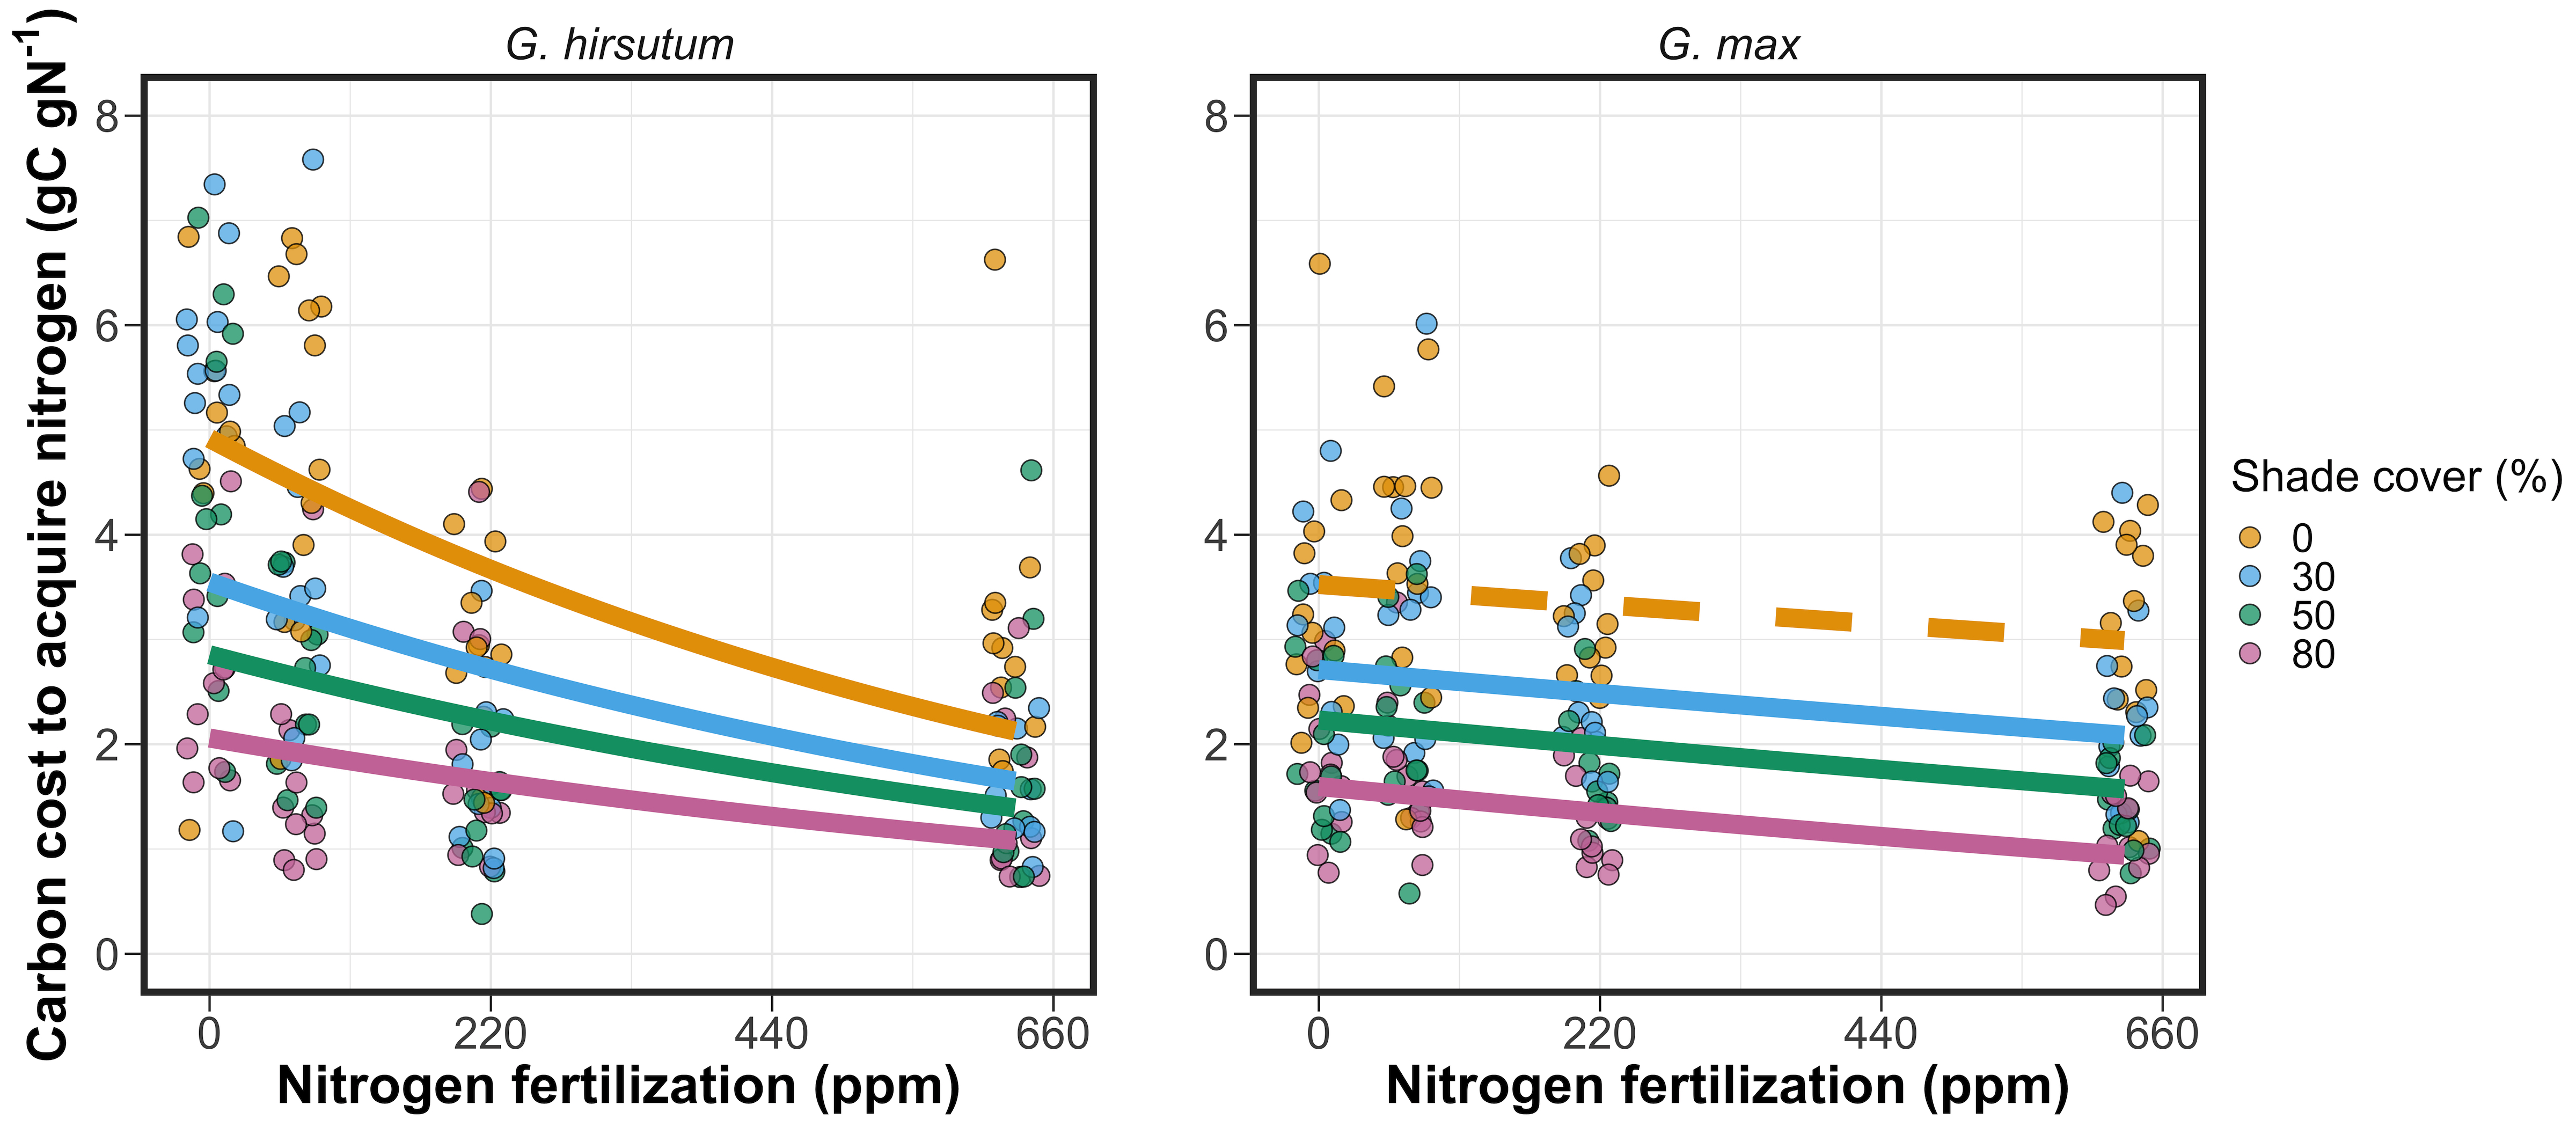
\includegraphics[width=\columnwidth]{ch2_LxN_Greenhouse/figs/fig1_ncost.jpg}
    \centering
    \caption[Effects of shade cover and nitrogen fertilization on plant carbon costs to acquire nitrogen in \textit{G. hirsutum} and \textit{G. max}]{Effects of shade cover and nitrogen fertilization on plant carbon costs to acquire nitrogen in \textit{G. hirsutum} (left panel) and \textit{G. max} (right panel). Nitrogen fertilization treatments are represented on the x-axis. Shade cover treatments are represented through colored points and trendlines. Trendlines were created by back-transforming predicted marginal mean values across the range in x-axis values using the `emmeans’ function in the `emmeans’ R package \shortcite{Lenth2019}. Specifically, carbon costs to acquire nitrogen were natural-log transformed for \textit{G. hirsutum} and square root transformed in \textit{G. max}. Points are jittered across the x-axis for visibility. Yellow points and trendlines represent the 0\% shade cover treatment, blue points and trendlines represent the 30\% shade cover treatment, green points and trendlines represent the 50\% shade cover treatment, and purple points and trendlines represent the 80\% shade cover treatment. Solid trendlines indicate slopes that are significantly different from zero (Tukey: \textit{p}<0.05), while dashed trendlines indicate slopes that are not statistically different from zero.}
    \label{fig:figure2.1}
\end{figure}
\end{landscape}
\clearpage

\newpage
\subsection{\textit{Whole plant nitrogen biomass}}
\noindent Whole plant nitrogen biomass in \textit{G. hirsutum} was driven by an interaction between light availability and nitrogen fertilization (\textit{p}=0.001; Table \ref{tab:table2.1}; Fig. \ref{fig:figure2.2}). This interaction indicated a greater stimulation of whole-plant nitrogen biomass by nitrogen fertilization as light levels increased (Table \ref{tab:table2.1}; Fig. \ref{fig:figure2.2}).

Whole plant nitrogen biomass in \textit{G. max} increased with increasing light availability (\textit{p}<0.001) and nitrogen fertilization (\textit{p}<0.001), with no interaction between light availability and nitrogen fertilization (\textit{p}=0.231; Table \ref{tab:table2.1}; Fig. \ref{fig:figure2.2}).

\newpage
\begin{landscape}
\begin{figure}
    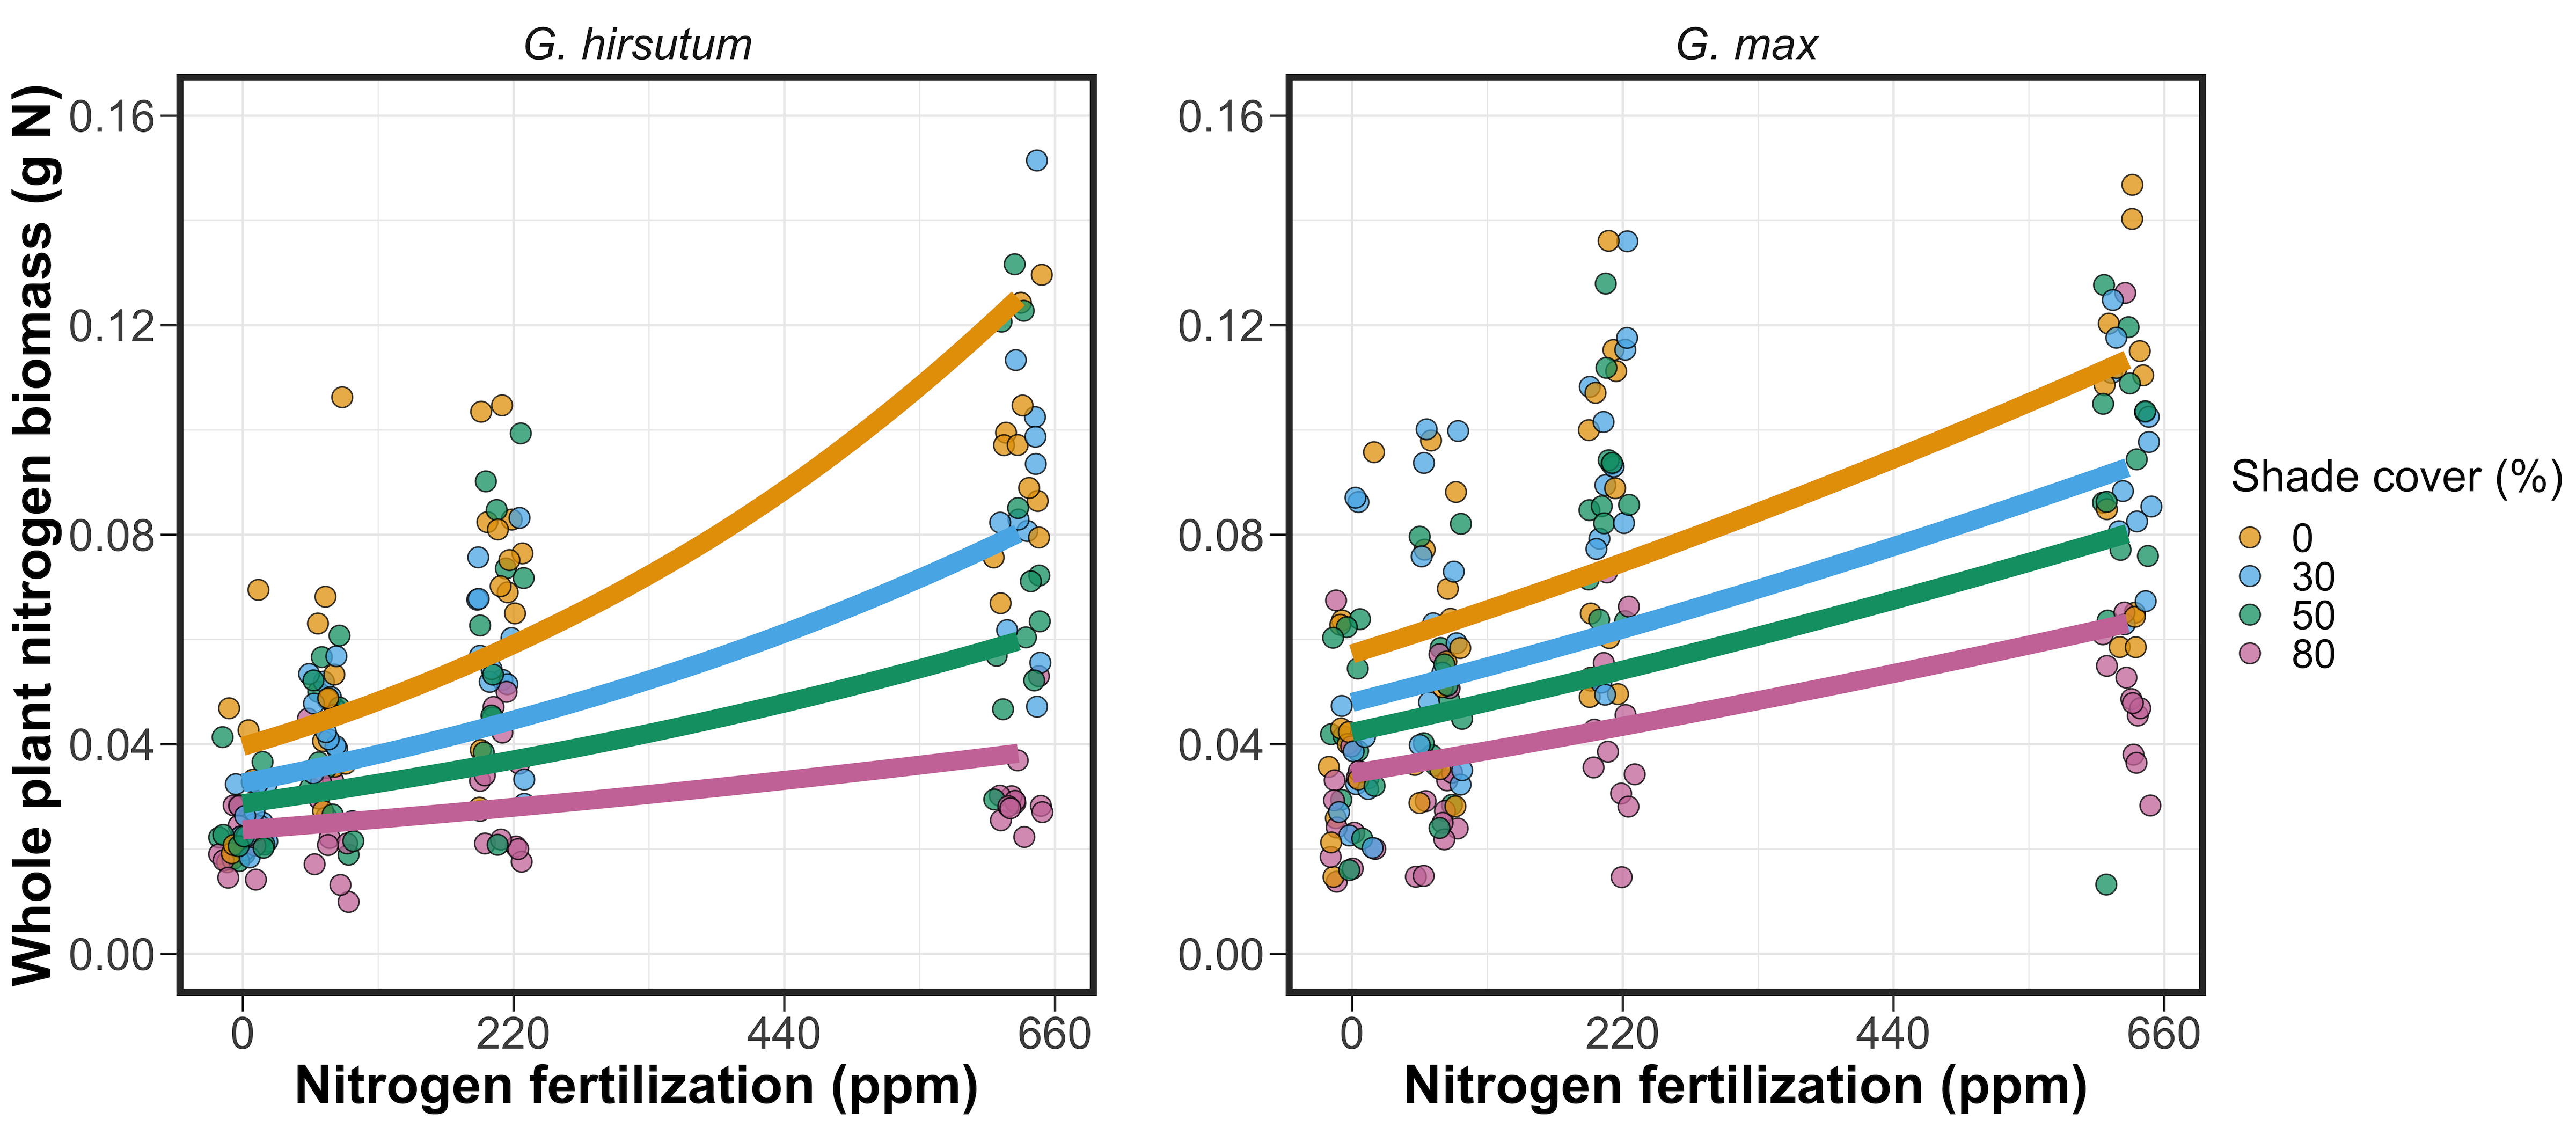
\includegraphics[width = \columnwidth]{ch2_LxN_Greenhouse/figs/fig2_nacq.jpg}
    \centering
    \caption[Effects of shade cover and nitrogen fertilization on whole-plant nitrogen biomass in \textit{G. hirsutum} and \textit{G. max}]{Effects of shade cover and nitrogen fertilization on whole-plant nitrogen biomass in \textit{G. hirsutum} (left panel) and \textit{G. max} (right panel). Whole-plant nitrogen biomass is the denominator of the carbon cost to acquire nitrogen calculation. Nitrogen fertilization treatments are represented on the x-axis. Shade cover treatments are represented through colored points and trendlines. Trendlines were created by back-transforming predicted marginal mean values across the range in x-axis values using the `emmeans’ function in the `emmeans’ R package \shortcite{Lenth2019}. Specifically, whole plant nitrogen biomass was natural-log transformed for \textit{G. hirsutum} and square root transformed in \textit{G. max}. Points are jittered across the x-axis for visibility. Points and trendlines are as explained in Fig. \ref{fig:figure2.1}. Solid trendlines indicate slopes that are significantly different from zero (Tukey: \textit{p}<0.05), while dashed trendlines indicate slopes that are not statistically different from zero.}
    \label{fig:figure2.2}
    \small
\end{figure}
\end{landscape}
\clearpage

\newpage
\subsection{\textit{Root carbon biomass}}
\noindent Root carbon biomass in \textit{G. hirsutum} significantly increased with increasing light availability (\textit{p}<0.001; Table \ref{tab:table2.1}; Fig. \ref{fig:figure2.3}) and marginally increased with nitrogen fertilization (\textit{p}=0.089; Table \ref{tab:table2.1}; Fig. \ref{fig:figure2.3}). There was also a marginal interaction between light availability and nitrogen fertilization (\textit{p}=0.076; Table \ref{tab:table2.1}), driven by an increase in the positive response of root carbon biomass to increasing nitrogen fertilization as light availability increased (Table \ref{tab:table2.3}). This pattern resulted in significantly positive trends between root carbon biomass and nitrogen fertilization in the two highest light treatments (Tukey: \textit{p}<0.05 in both cases; Table \ref{tab:table2.3}; Fig. \ref{fig:figure2.3}) and no effect of nitrogen fertilization in the two lowest light treatments (Tukey: \textit{p}>0.05 in both cases; Table \ref{tab:table2.3}; Fig. \ref{fig:figure2.3}). 

There was an interaction between light availability and nitrogen fertilization on root carbon biomass in \textit{G. max} (\textit{p}=0.001; Table \ref{tab:table2.1}; Fig. \ref{fig:figure2.3}). Post-hoc analyses indicated that the positive effects of nitrogen fertilization on \textit{G. max} root carbon biomass increased with increasing light availability (Table \ref{tab:table2.3}; Fig. \ref{fig:figure2.3}). There were also positive individual effects of increasing nitrogen fertilization (\textit{p}<0.001; Table \ref{tab:table2.3}) and light availability (\textit{p}<0.001; Table \ref{tab:table2.3}) on \textit{G. max} root carbon biomass (Table \ref{tab:table2.1}; Fig. \ref{fig:figure2.3}).

\newpage
\begin{landscape}
\begin{figure}
    \centering
    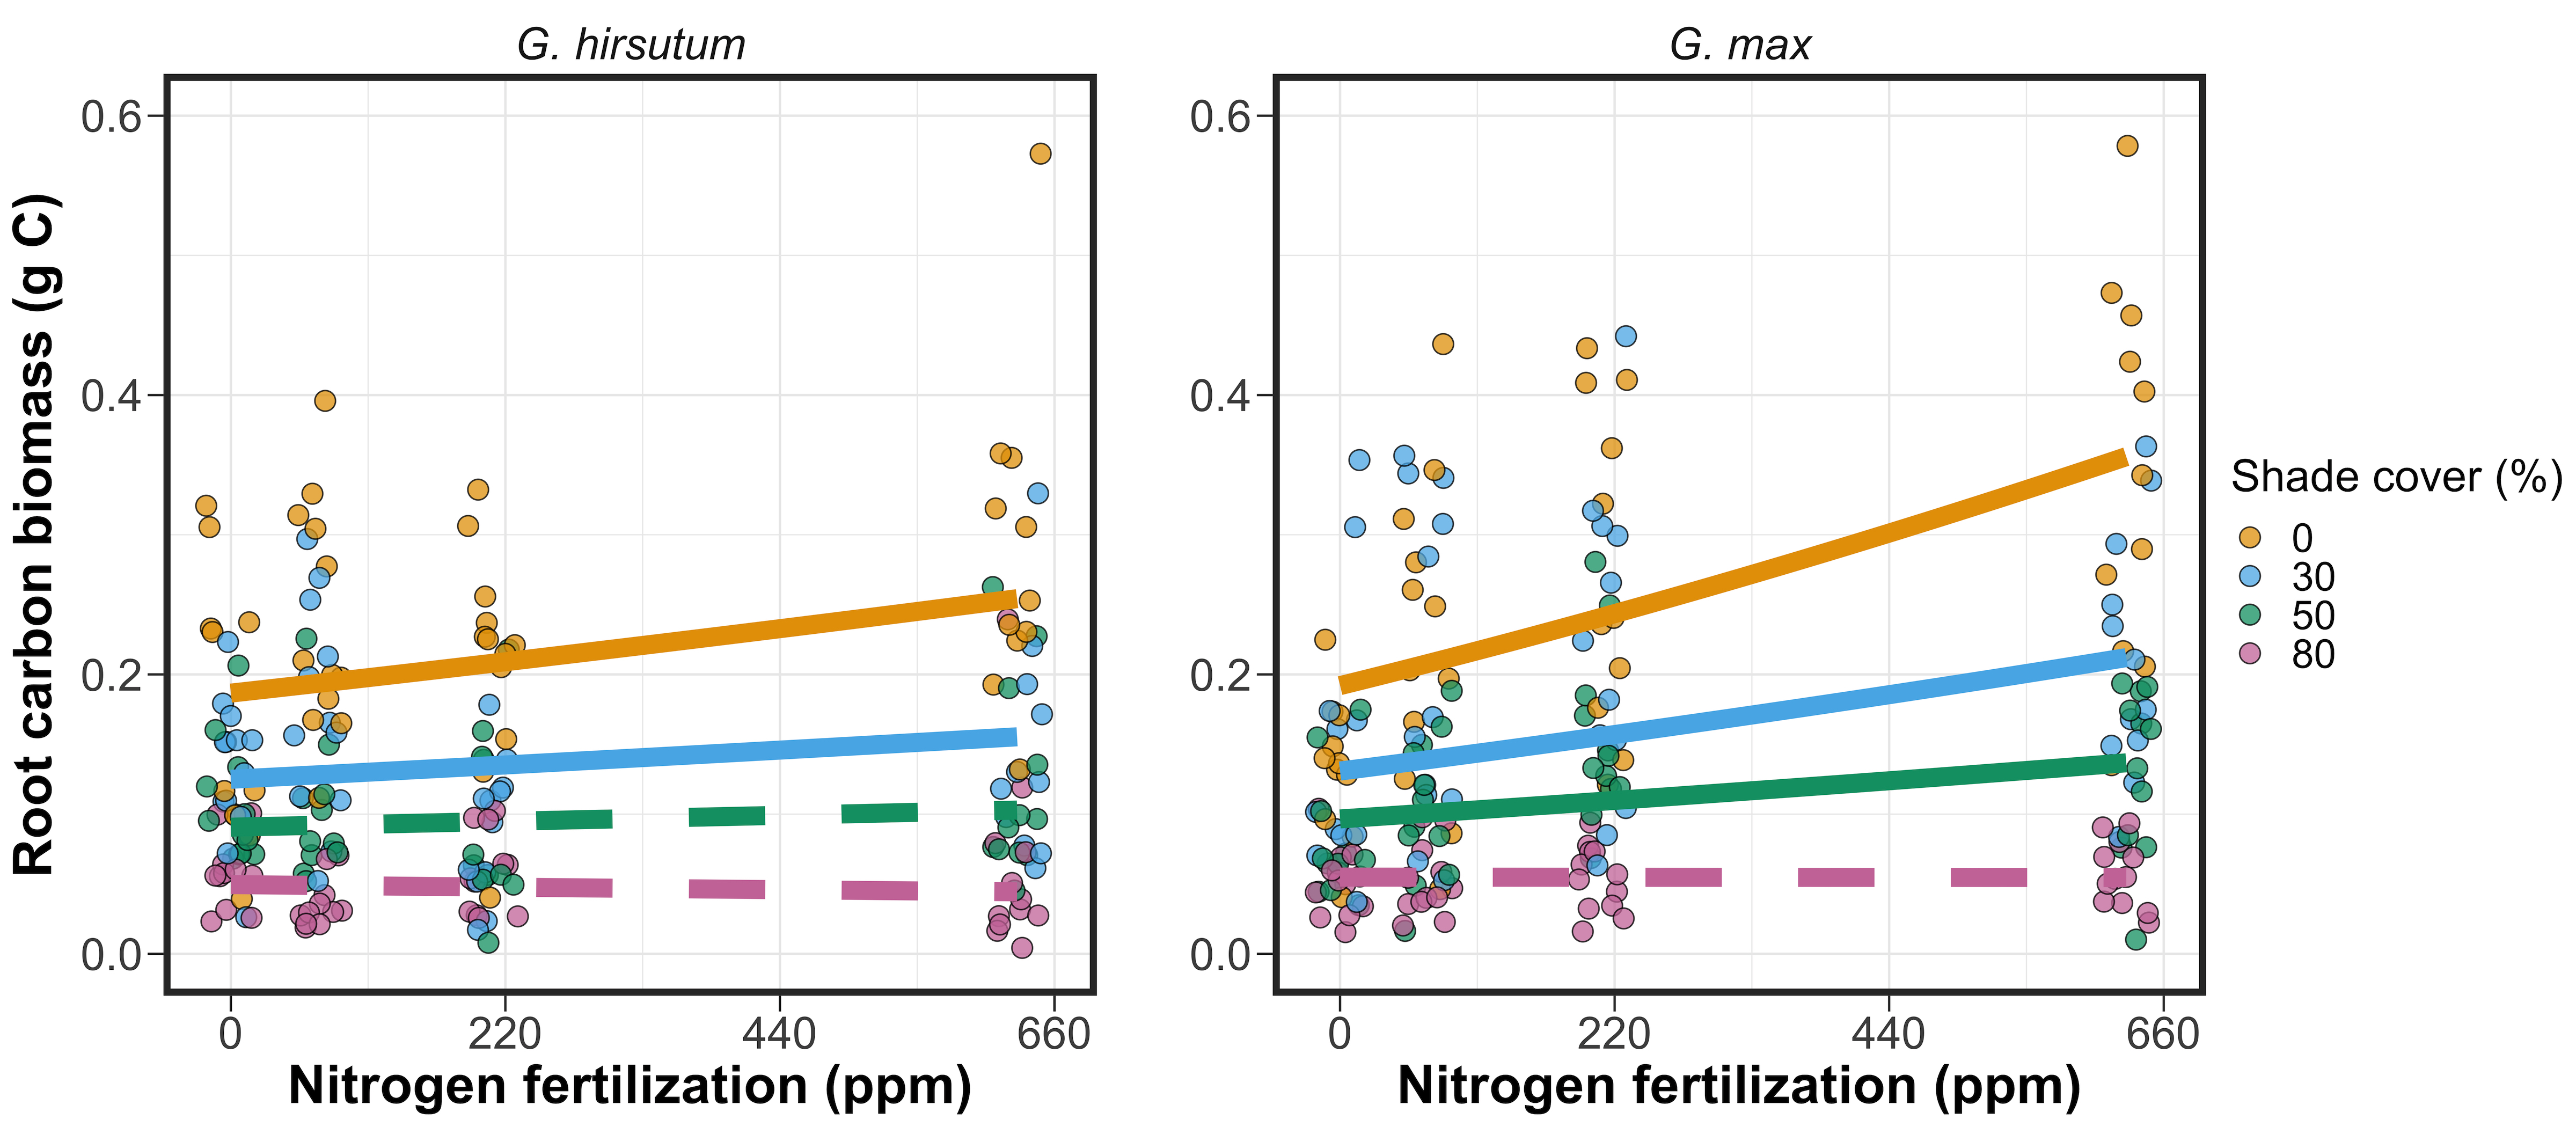
\includegraphics[width = \columnwidth]{ch2_LxN_Greenhouse/figs/fig3_rootCarbon.jpg}
    \caption[Effects of shade cover and nitrogen fertilization on root carbon biomass in \textit{G. hirsutum} and \textit{G. max}]{Effects of shade cover and nitrogen fertilization on root carbon biomass in \textit{G. hirsutum} (left panel) and \textit{G. max} (right panel). Root carbon biomass is the numerator of the carbon cost to acquire nitrogen calculation. Nitrogen fertilization treatments are represented on the x-axis. Shade cover treatments are represented through colored points and trendlines. Trendlines were created by back-transforming predicted marginal mean values across the range in x-axis values using the `emmeans’ function in the `emmeans’ R package \shortcite{Lenth2019}. Specifically, root carbon biomass was square root transformed for both species. Points are jittered across the x-axis for visibility. Colored points and trendlines are as explained in Fig. \ref{fig:figure2.1}. Solid trendlines indicate slopes that are significantly different from zero (Tukey: \textit{p}<0.05), while dashed trendlines indicate slopes that are not statistically different from zero.}
    \label{fig:figure2.3}
\end{figure}
\end{landscape}
\clearpage

\newpage
\subsection{\textit{Root nodule biomass}}
\noindent Root nodule biomass in \textit{G. max} increased with increasing light availability (\textit{p}< 0.001; Table \ref{tab:table2.2}; Fig. \ref{fig:figure2.4}a) and decreased with increasing nitrogen fertilization (\textit{p}<0.001; Table \ref{tab:table2.2}; Fig. \ref{fig:figure2.4}a). There was no interaction between nitrogen fertilization and light availability (\textit{p}=0.133; Table \ref{tab:table2.2}; Fig. \ref{fig:figure2.4}a). The ratio of root nodule biomass to root biomass did not change in response to light availability (\textit{p}=0.481; Table \ref{tab:table2.2}; Fig. \ref{fig:figure2.4}b) but decreased with increasing nitrogen fertilization (\textit{p}<0.001; Table \ref{tab:table2.2}; Fig. \ref{fig:figure2.4}b). There was no interaction between nitrogen fertilization and light availability on the ratio of root nodule biomass to root biomass (\textit{p}=0.621; Table \ref{tab:table2.2}; Fig. \ref{fig:figure2.4}b).

\newpage
\begin{landscape}
\begin{table}
    \caption[Analysis of variance results exploring effects of light availability, nitrogen fertilization, and their interactions on \textit{G. max} root nodule biomass and the ratio of root nodule biomass to root biomass]{Analysis of variance results exploring effects of light availability, nitrogen fertilization, and their interactions on \textit{G. max} root nodule biomass (g) and the ratio of root nodule biomass to root biomass (g g$^{-1}$)$^*$}
    \centering
    %\resizebox{\columnwidth}{!}{
    \begin{tabular}{p{2.4cm}p{0.5cm}p{2cm}p{1.5cm}p{1.5cm}p{2cm}p{1.5cm}p{1.5cm}}
        && 
        \multicolumn{3}{l}{Nodule biomass} 
        & \multicolumn{3}{l}{Nodule biomass: root biomass} 
        \\
        \hline
        & \multicolumn{1}{r}{df}
        & \multicolumn{1}{r}{Coefficient}   & \multicolumn{1}{r}{$\chi^{2}$}        & \multicolumn{1}{r}{\textit{p}}
        & \multicolumn{1}{r}{Coefficient}   & \multicolumn{1}{r}{$\chi^{2}$}        & \multicolumn{1}{r}{\textit{p}}
        \\
        \hline
        
        (Intercept)
        && \multicolumn{1}{r}{$3.02*10^{-1}$}        & \multicolumn{1}{r}{-}                 & \multicolumn{1}{r}{-}
        & \multicolumn{1}{r}{$4.48*10^{-1}$}         & \multicolumn{1}{r}{-}                 & \multicolumn{1}{r}{-} 
        \\
    
        Light (L) & \multicolumn{1}{r}{1}
        & \multicolumn{1}{r}{$-1.81*10^{-3}$}     & \multicolumn{1}{r}{72.964}            & \multicolumn{1}{r}{\textbf{<0.001}}
        & \multicolumn{1}{r}{$-8.76*10^{-5}$}     & \multicolumn{1}{r}{0.496}             & \multicolumn{1}{r}{0.481} 
        \\
    
        Nitrogen (N) & \multicolumn{1}{r}{1}
        & \multicolumn{1}{r}{$-2.83*10^{-4}$}     & \multicolumn{1}{r}{115.377}           & \multicolumn{1}{r}{\textbf{<0.001}}
        & \multicolumn{1}{r}{$-5.09*10^{-4}$}     & \multicolumn{1}{r}{156.476}           & \multicolumn{1}{r}{\textbf{<0.001}} 
        \\
    
        L*N & \multicolumn{1}{r}{1}
        &  \multicolumn{1}{r}{$1.14*10^{-6}$}     &   \multicolumn{1}{r}{2.226}           & \multicolumn{1}{r}{0.133}
        & \multicolumn{1}{r}{$-7.30*10^{-7}$}     &   \multicolumn{1}{r}{0.244}           & \multicolumn{1}{r}{0.621}
        \\
        \hline
        \\
    \end{tabular}%}
    \label{tab:table2.2}
\end{table}
\begin{singlespace}
    \noindent $^*$Significance determined using Wald’s $\chi^{2}$ tests ($\alpha$=0.05). \textit{P}-values less than 0.05 are in bold. Negative coefficients for light treatments indicate a positive effect of increasing light availability on all response variables, as light availability is treated as percent shade cover in all linear mixed-effects models. Root nodule biomass and nodule biomass: root biomass models were only constructed for \textit{G. max} because \textit{G. hirsutum} was not inoculated with \textit{B. japonicum} and is not capable of forming root nodules.
\end{singlespace}
\end{landscape}
\clearpage

\newpage
\begin{landscape}
    \begin{table}
        \caption[Slopes of the regression line describing the relationship between each dependent variable and nitrogen fertilization at each light level]{Slopes of the regression line describing the relationship between each dependent variable and nitrogen fertilization at each light level$^*$}
        \centering
        \resizebox{\columnwidth}{!}{
            \begin{tabular}{p{2cm}p{3.2cm}p{3.2cm}p{3.2cm}p{3.2cm}p{3.2cm}}
            \hline
            \begin{tabular}[c]{@{}l@{}}Shade\\ cover\end{tabular} 
            & \begin{tabular}[c]{@{}l@{}}Carbon cost to\\ acquire nitrogen\end{tabular} 
            & \begin{tabular}[c]{@{}l@{}}Whole plant\\ nitrogen biomass\end{tabular}
            & \begin{tabular}[c]{@{}l@{}}Belowground\\ carbon biomass\end{tabular}
            & \begin{tabular}[c]{@{}l@{}}Root nodule\\ biomass\end{tabular}
            & \begin{tabular}[c]{@{}l@{}}Nodule biomass:\\ root biomass\end{tabular} 
            \\
            \hline
             
            \multicolumn{1}{l}{\textit{G. hirsutum}} \\
            \multicolumn{1}{r}{0\%}
            &  \multicolumn{1}{r}{\textbf{$-1.34*10^{-3\mathrm{a}}$}}
            &  \multicolumn{1}{r}{\textbf{$1.83*10^{-3\mathrm{a}}$}}
            &  \multicolumn{1}{r}{\textbf{$1.15*10^{-4\mathrm{b}}$}}
            &  \multicolumn{1}{r}{-}
            &  \multicolumn{1}{r}{-}
            \\
            \multicolumn{1}{r}{30\%}                     
            &  \multicolumn{1}{r}{\textbf{$-1.22*10^{-3\mathrm{a}}$}}
            &  \multicolumn{1}{r}{\textbf{$1.43*10^{-3\mathrm{a}}$}}
            &  \multicolumn{1}{r}{\textbf{$1.17*10^{-4\mathrm{b}}$}}
            &  \multicolumn{1}{r}{-}
            &  \multicolumn{1}{r}{-}
            \\
            \multicolumn{1}{r}{50\%}
            &  \multicolumn{1}{r}{\textbf{$-1.14*10^{-3\mathrm{a}}$}}
            &  \multicolumn{1}{r}{\textbf{$1.17*10^{-3\mathrm{a}}$}}
            &  \multicolumn{1}{r}{$3.12*10^{-5\mathrm{b}}$}
            &  \multicolumn{1}{r}{-}
            &  \multicolumn{1}{r}{-}
            \\
            \multicolumn{1}{r}{80\%}
            &  \multicolumn{1}{r}{\textbf{$-1.02*10^{-3\mathrm{a}}$}}
            &  \multicolumn{1}{r}{\textbf{$7.66*10^{-4\mathrm{a}}$}}
            &  \multicolumn{1}{r}{$-1.89*10^{-6\mathrm{b}}$}
            &  \multicolumn{1}{r}{-}
            &  \multicolumn{1}{r}{-}
            \\
            &&&& 
            \\
            \multicolumn{1}{l}{\textit{G. max}}
            \\
            \multicolumn{1}{r}{0\%}
            &  \multicolumn{1}{r}{$-2.35*10^{-4\mathrm{b}}$}
            &  \multicolumn{1}{r}{\textbf{$1.55*10^{-5\mathrm{b}}$}}
            &  \multicolumn{1}{r}{\textbf{$2.51*10^{-4\mathrm{b}}$}}
            &  \multicolumn{1}{r}{\textbf{$-2.83*10^{-4\mathrm{b}}$}}
            &  \multicolumn{1}{r}{\textbf{$-5.09*10^{-4\mathrm{b}}$}}
            \\
              
            \multicolumn{1}{r}{30\%}
            &  \multicolumn{1}{r}{\textbf{$-3.22*10^{-4\mathrm{b}}$}}
            &  \multicolumn{1}{r}{\textbf{$1.35*10^{-5\mathrm{b}}$}}
            &  \multicolumn{1}{r}{\textbf{$1.57*10^{-4\mathrm{b}}$}}
            &  \multicolumn{1}{r}{\textbf{$-2.49*10^{-4\mathrm{b}}$}}
            &  \multicolumn{1}{r}{\textbf{$-5.31*10^{-4\mathrm{b}}$}}
            \\
              
            \multicolumn{1}{r}{50\%}
            &  \multicolumn{1}{r}{\textbf{$-3.80*10^{-4\mathrm{b}}$}}
            &  \multicolumn{1}{r}{\textbf{$1.23*10^{-5\mathrm{b}}$}}
            &  \multicolumn{1}{r}{\textbf{$9.37*10^{-5\mathrm{b}}$}}
            &  \multicolumn{1}{r}{\textbf{$-2.26*10^{-4\mathrm{b}}$}}
            &  \multicolumn{1}{r}{\textbf{$-5.45*10^{-4\mathrm{b}}$}}
            \\
              
            \multicolumn{1}{r}{80\%}
            &  \multicolumn{1}{r}{\textbf{$-4.66*10^{-4\mathrm{b}}$}}
            &  \multicolumn{1}{r}{\textbf{$1.04*10^{-5\mathrm{b}}$}}
            &  \multicolumn{1}{r}{$-9.95*10^{-7\mathrm{b}}$}
            &  \multicolumn{1}{r}{\textbf{$-1.92*10^{-4\mathrm{b}}$}}
            &  \multicolumn{1}{r}{\textbf{$-5.67*10^{-4\mathrm{b}}$}}
            \\
            \hline
        \end{tabular}}
        \label{tab:table2.3}
    \end{table}
\begin{singlespace}
    \noindent $^*$ Slopes represent estimated marginal mean slopes from linear mixed-effects models described in the Methods. Slopes were calculated using the ‘emmeans’ R package \shortcite{Lenth2019}. Superscripts indicate slopes fit to natural-log ($^\mathrm{a}$) or square root ($^\mathrm{b}$) transformed data. Slopes statistically different from zero (Tukey: \textit{p}<0.05) are indicated in bold. Marginally significant slopes (Tukey: 0.05<\textit{p}<0.1) are italicized.
\end{singlespace}
\end{landscape}
\clearpage

\newpage
\begin{landscape}

\begin{figure}
    \centering
    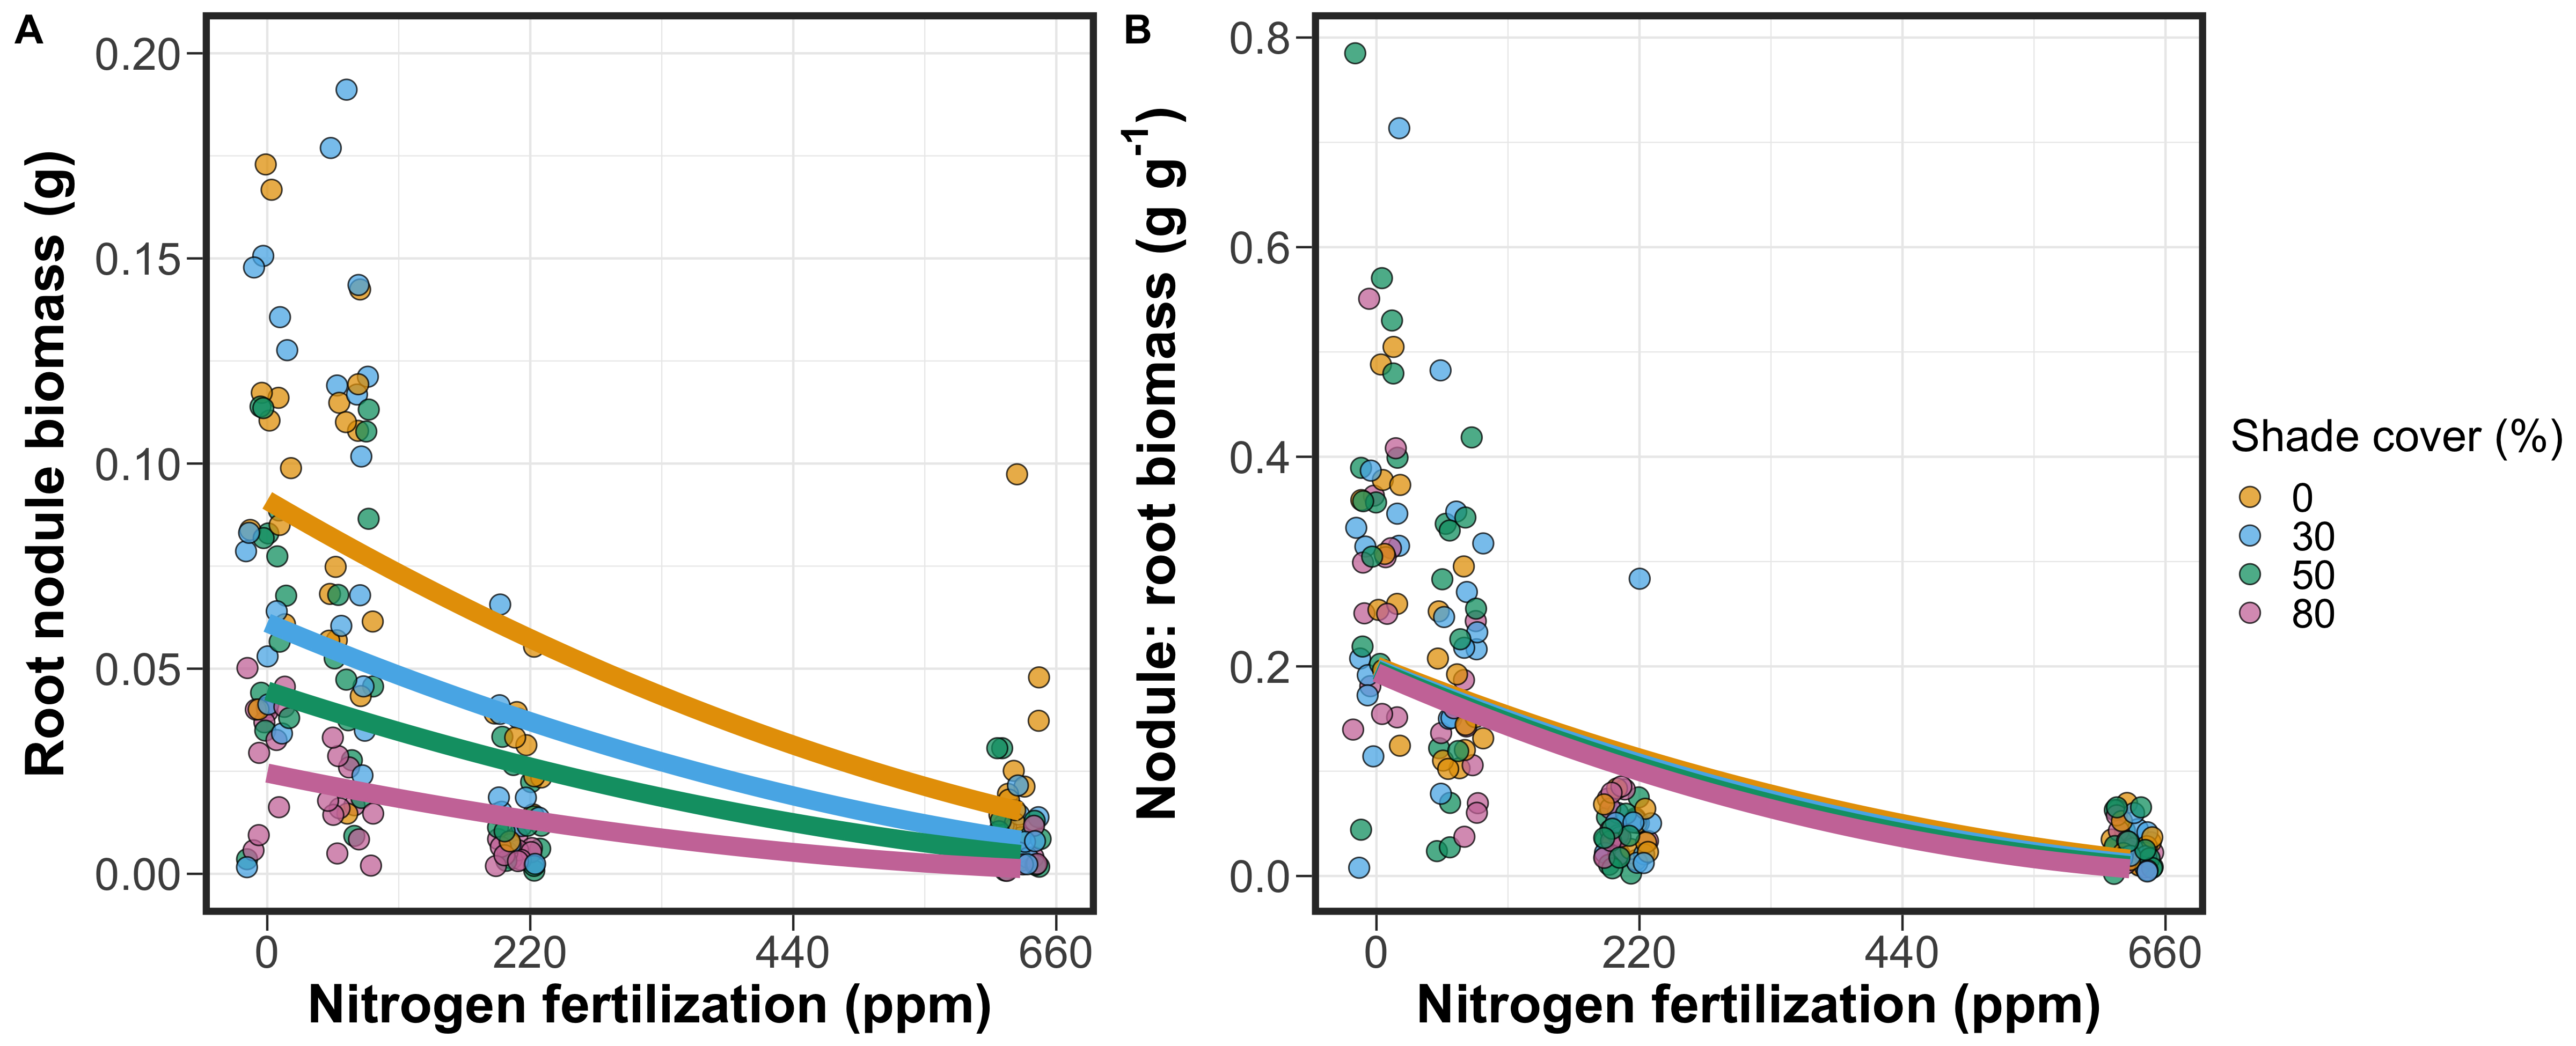
\includegraphics[width = \columnwidth]{ch2_LxN_Greenhouse/figs/fig4_nodwgt.jpg}
    \caption[Effects of shade cover and nitrogen fertilization on root nodule biomass and the ratio of root nodule biomass to root biomass in \textit{G. max}.]{Effects of shade cover and nitrogen fertilization on root nodule biomass (A) and the ratio of root nodule biomass to root biomass (B) in \textit{G. max}. Nitrogen fertilization treatments are represented on the x-axis. Shade cover treatments are represented through colored points and trendlines. Trendlines were created by back-transforming predicted marginal mean values across the range in x-axis values using the `emmeans’ function in the `emmeans’ R package \shortcite{Lenth2019}. Specifically, root nodule biomass and the ratio of root nodule biomass to root biomass were each square root transformed. Points are jittered across the x-axis for visibility. Colored points and trendlines are as explained in Fig. \ref{fig:figure2.1}. Solid trendlines indicate slopes that are significantly different from zero (Tukey: \textit{p}<0.05), while dashed trendlines indicate slopes that are not statistically different from zero.}
    \label{fig:figure2.4}
\end{figure}
\end{landscape}
\clearpage

\section{Discussion}
\noindent In this chapter, I determined the effects of light availability and soil nitrogen fertilization on root mass carbon costs to acquire nitrogen in \textit{G. hirsutum} and \textit{G. max}. In support of my hypotheses, I found that carbon costs to acquire nitrogen generally increased with increasing light availability and decreased with increasing soil nitrogen fertilization in both species. These findings suggest that carbon costs to acquire nitrogen are determined by factors that influence plant nitrogen demand and soil nitrogen availability. In contrast to my second hypothesis, root nodulation data suggested that \textit{G. max} and \textit{G. hirsutum} achieved similar directional carbon cost responses to nitrogen fertilization despite a likely shift in \textit{G. max} allocation from nodulation to root biomass along the nitrogen fertilization gradient.

Both \textit{G. max} and \textit{G. hirsutum} experienced an increase in carbon costs to acquire nitrogen due to increasing light availability. These patterns were driven by a larger increase in root carbon biomass than whole-plant nitrogen biomass. Increases in root carbon biomass due to factors that increase plant nitrogen demand are a commonly observed pattern, as carbon allocated belowground provides substrate needed to produce and maintain structures that satisfy aboveground plant nitrogen demand \shortcite{Nadelhoffer1992,Giardina2005,Raich2014}. Findings suggest that plants allocate relatively more carbon for acquiring nitrogen when demand increases over short temporal scales, which may cause a temporary state of diminishing return due to asynchrony between belowground carbon and whole-plant nitrogen responses to plant nitrogen demand \shortcite{Kulmatiski2017,Noyce2019}. These responses might be attributed to a temporal lag associated with producing structures that enhance nitrogen acquisition. For example, fine roots \shortcite{Matamala2000,Norby2004,Arndal2018} and root nodules \shortcite{Parvin2020} take time to build and first require the construction of coarse roots. Thus, full nitrogen returns from these investments may not occur immediately \shortcite{Kayler2010,Kayler2017}, and may vary by species acquisition strategy. I speculate that increases in nitrogen acquisition from a given carbon investment may occur beyond the 5-week scope of this experiment. A similar study conducted over a longer temporal scale would address this.

Increasing soil nitrogen fertilization generally decreased carbon costs to acquire nitrogen in both species. These patterns were driven by a larger increase in whole-plant nitrogen biomass than root carbon biomass. In \textit{G. hirsutum}, reductions in carbon costs to acquire nitrogen may have been due to an increase in per-root nitrogen uptake, allowing individuals to maximize the amount of nitrogen acquired from a belowground carbon investment. Interestingly, increased soil nitrogen fertilization increased whole-plant nitrogen biomass in \textit{G. max} despite reductions in root nodule biomass that likely reduced the nitrogen-fixing capacity of \textit{G. max} \shortcite{Andersen2005,Munoz2016}. While reductions in root nodulation due to increased soil nitrogen availability are commonly observed \shortcite{Gibson1985,Fujikake2003}, root nodulation responses were observed in tandem with increased root carbon biomass, implying that \textit{G. max} shifted relative carbon allocation from nitrogen fixation to soil nitrogen acquisition \shortcite{Markham2007,Dovrat2020}. This was likely because there was a reduction in the carbon cost advantage of acquiring fixed nitrogen relative to soil nitrogen, and suggests that species capable of associating with symbiotic nitrogen-fixing bacteria shift their relative nitrogen acquisition pathway to optimize nitrogen uptake \shortcite{Rastetter2001}. Future studies should investigate these patterns with a larger quantity of phylogenetically related species, or different varieties of a single species that differ in their ability to form associations with symbiotic nitrogen-fixing bacteria to more directly test the impact of nitrogen fixation on the patterns observed in this study.

Carbon costs to acquire nitrogen are subsumed in the general discussion of economic analogies to plant resource uptake \shortcite{Bloom1985,Rastetter2001,Vitousek2002,Phillips2013,Terrer2018,Henneron2020}. Despite this, terrestrial biosphere models rarely include costs of nitrogen acquisition to predict plant nitrogen uptake. There is currently one plant resource uptake model, the Fixation and Uptake of Nitrogen model (FUN), that quantitatively predicts carbon costs to acquire nitrogen within a framework for predicting plant nitrogen uptake for different nitrogen acquisition strategies \shortcite{Fisher2010,Brzostek2014FUN2}. Iterations of FUN are currently coupled to two terrestrial biosphere models: the Community Land Model 5.0 and the Joint UK Land Environment Simulator \shortcite{Clark2011,Shi2016,Lawrence2019}. Recent work suggests that coupling FUN to CLM 5.0 caused a large overprediction of plant nitrogen uptake associated with nitrogen fixation \shortcite{Davies-Barnard2020} compared to other terrestrial biosphere model products. Thus, empirical data from manipulative experiments that explicitly quantify carbon costs to acquire nitrogen in species capable of associating with nitrogen-fixing bacteria across different environmental contexts is an important step toward identifying potential biases in models such as FUN.

These findings support the FUN formulation of carbon costs to acquire nitrogen in response to soil nitrogen availability. FUN calculates carbon costs to acquire nitrogen based on the sum of carbon costs to acquire nitrogen via nitrogen fixation, mycorrhizal active uptake, non-mycorrhizal active uptake, and retranslocation \shortcite{Fisher2010,Brzostek2014FUN2}. Carbon costs to acquire nitrogen via mycorrhizal or non-mycorrhizal active uptake pathways are derived as a function of nitrogen availability, root biomass, and two parameterized values based on nitrogen acquisition strategy \shortcite{Brzostek2014FUN2}. Due to this, FUN simulates a net decrease in carbon costs to acquire nitrogen with increasing nitrogen availability for mycorrhizal and non-mycorrhizal active uptake pathways, assuming constant root biomass. This was a pattern I observed in \textit{G. hirsutum} regardless of light availability. In contrast, FUN would not simulate a net change in carbon costs to acquire nitrogen via nitrogen fixation due to nitrogen availability. This is because carbon costs to acquire nitrogen via nitrogen fixation are derived from a well established function of soil temperature, which is independent of soil nitrogen availability \shortcite{Houlton2008,Fisher2010}. I observed a net reduction in carbon costs to acquire nitrogen in \textit{G. max}, except when individuals were grown under 0\% shade cover. While a net reduction of carbon costs in response to nitrogen fertilization runs counter to nitrogen fixation carbon costs simulated by FUN, these patterns were likely because \textit{G. max} individuals switched their primary mode of nitrogen acquisition from symbiotic nitrogen fixation to a non-symbiotic active uptake pathway.

The metric used in this study to determine carbon costs to acquire nitrogen has several limitations. Most notably, this metric uses root carbon biomass as a proxy for estimating the amount of carbon spent on nitrogen acquisition. Although it is true that most carbon allocated belowground has at least an indirect structural role in acquiring soil resources, it remains unclear whether this assumption holds true for species that acquire nitrogen via symbiotic nitrogen fixation. I also cannot quantify carbon lost through root exudates or root turnover, which may increase due to factors that increase plant nitrogen demand \shortcite{Tingey2000,Phillips2011}, and can increase the magnitude of available nitrogen from soil organic matter through priming effects on soil microbial communities \shortcite{Uselman2000,Bengtson2012}. It is also not clear whether these assumptions hold under all environmental conditions, such as those that shift belowground carbon allocation toward a different mode of nitrogen acquisition \shortcite{Taylor2018,Friel2019} or between species with different acquisition strategies. In this study, increasing soil nitrogen fertilization increased carbon investment to roots relative to carbon transferred to root nodules. By assuming that carbon allocated to root carbon was proportional to carbon allocated to root nodules across all treatment combinations, these observed responses to soil nitrogen fertilization were likely to be overestimated in \textit{G. max}. I encourage future research to quantify these carbon fates independently.

Carbon costs to acquire nitrogen decreased with increasing fertilization more strongly in \textit{G. hirsutum} than \textit{G. max}, a pattern that may have been driven by decreased investment to symbiotic nitrogen-fixing bacteria with increasing fertilization in \textit{G. max}. However, species differed by more than just acquisition strategy, as \textit{G. hirsutum} is a woody perennial species and \textit{G. max} is a herbaceous annual species. Therefore, assigning causality to the stronger reduction in costs of nitrogen acquisition in \textit{G. hirsutum} is a challenge, and only provides anecdotal evidence that such patterns are generalizable across species. As previously mentioned, future experiments should attempt to measure such responses across a wider range of phylogenetically similar species or in a single species while explicitly controlling the source of nitrogen uptake.

Researchers conducting pot experiments must carefully choose pot volume to minimize the likelihood of growth limitations induced by pot volume \shortcite{Poorter2012}. \shortciteN{Poorter2012} indicate that researchers are likely to avoid growth limitations associated with pot volume if measurements are collected when the plant biomass:pot volume ratio is less than 1 g L$^{-1}$. In this experiment, all treatment combinations in both species had biomass:pot volume ratios less than 1 g L$^{-1}$ except for \textit{G. max} and \textit{G. hirsutum} that were grown under 0\% shade cover and had received 630 ppm N. Specifically, \textit{G. max} and \textit{G. hirsutum} had average respective biomass:pot volume ratios of 1.24$\pm$0.07 g L$^{-1}$ and 1.34$\pm$0.13 g L$^{-1}$, when grown under 0\% shade cover and received 630 ppm N (Table \ref{table:tab.a2}, \ref{table:tab.a3}; Fig. \ref{fig:figure.a1}). If growth in this treatment combination was limited by pot volume, then individuals may have had larger carbon costs to acquire nitrogen than would be expected if they were grown in larger pots. This pot volume induced growth limitation could cause a reduction in per-root nitrogen uptake associated with more densely packed roots, which could reduce the positive effect of nitrogen fertilization on whole-plant nitrogen biomass relative to root carbon biomass \shortcite{Poorter2012}.

Pot size may have limited plant growth, which provides a possible explanation for the marginally insignificant effect of increasing nitrogen fertilization on \textit{G. max} carbon costs to acquire nitrogen when grown under 0\% shade cover. This is because the regression line describing the relationship between carbon costs to acquire nitrogen and nitrogen fertilization in \textit{G. max} grown under 0\% shade cover would have flattened if growth limitation had caused larger than expected carbon costs to acquire nitrogen in the 0\% shade cover, 630 ppm N treatment combination. This may have been exacerbated by the fact that \textit{G. max} likely shifted relative carbon allocation from nitrogen fixation to soil nitrogen acquisition, which could have increased the negative effect of more densely packed roots on nitrogen uptake. These patterns could have also occurred in \textit{G. hirsutum} grown under 0\% shade cover; however, there was no change in the effect of nitrogen fertilization on \textit{G. hirsutum} carbon costs to acquire nitrogen grown under 0\% shade cover relative to other shade cover treatments. Regardless, the possibility of growth limitation due to pot volume suggests that effects of increasing nitrogen fertilization on carbon costs to acquire nitrogen in both species grown under 0\% shade cover could have been underestimated. Follow-up studies using a similar experimental design with a larger pot volume would be necessary in order to determine whether these patterns were impacted by pot volume-induced growth limitation.

In conclusion, this chapter provides empirical evidence that carbon costs to acquire nitrogen are influenced by light availability and soil nitrogen fertilization in a species capable of acquiring nitrogen via symbiotic nitrogen fixation and a species not capable of forming such associations. We show that carbon costs to acquire nitrogen generally increase with increasing light availability and decrease with increasing nitrogen fertilization. This chapter provides important empirical data needed to evaluate the formulation of carbon costs to acquire nitrogen in terrestrial biosphere models, particularly carbon costs to acquire nitrogen that are associated with symbiotic nitrogen fixation. Findings broadly support the general formulation of these carbon costs in the FUN biogeochemical model in response to shifts in nitrogen availability. However, there is a need for future studies to explicitly quantify carbon costs to acquire nitrogen under different environmental contexts, over longer temporal scales, and using larger selections of phylogenetically related species. In addition, I suggest that future studies minimize the limitations associated with the metric used here by explicitly measuring belowground carbon fates independently.